% !TeX root = ../main.tex
\chapter{Introduction}\label{chapter:introduction}


\ac{VR} is a relatively new medium. Best practices are not set yet which leaves a lot of room for new methods and research. While common consumer \ac{VR} headsets (\acfp{HMD}) are rather similar, tracked hand controllers (\ac{VR}/hand/motion controllers) differ a lot as seen in Figure~\ref{fig:vr-controllers}.

\begin{figure}[H]
  \centering
  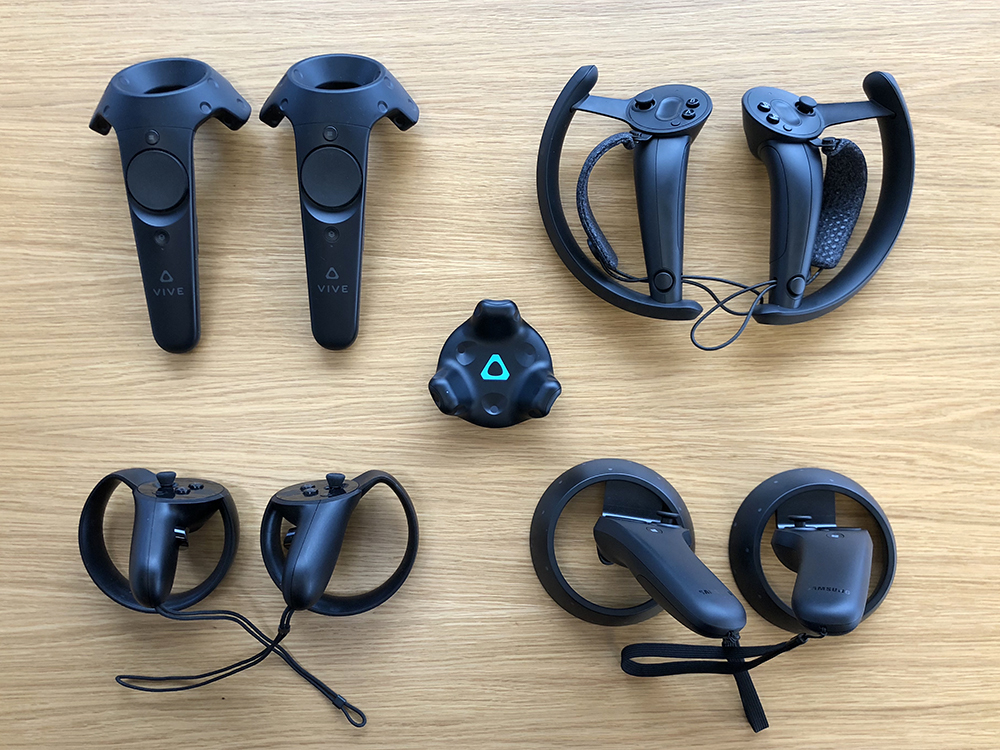
\includegraphics[width=12cm]{figures/vr_controllers.jpg}
  \caption[Collection of VR controllers]{A collection of different \ac{VR} controllers. From left to right, top to bottom: HTC VIVE Controllers, Valve Index Controllers (\enquote{Knuckles}), VIVE Tracker, Oculus Touch Controller, Samsung Odyssey Controllers.\source{\href{https://steamcommunity.com/games/250820/announcements/detail/1697188096865619876}{www.steamcommunity.com/games/\dots/announcements/\dots}}}\label{fig:vr-controllers}
\end{figure}



%\subsection{Virtual Reality}\label{subsection:virtual-reality}
